\chapter{Improvement of Visual Odometry}\label{Chap:Imp}
Above the procedure of self-localization was described in general. Both unscented Kalman filter and particle filter will require the pose information which provided by visual odometry part. So the accuracy of pose estimated by visual part will definitely have an obvious influence on the final result.
\clearpage
\section{Visual Odometry Procedure}
There are several sensors to acquire information from the environment on NAO: camera, microphone and sonar. From them only the camera is adopted, since the environment of the soccer match will be quite complicated, for example:
\begin{itemize}
    \item The white border lines and green field are on the same plane.
    \item The goal posts are perhaps too far away from the robots sometimes.
    \item There are 6 moving robots on the field, which the opponents are distinguished from our teammates only by colors.
    \item The ball is small and the detection of a ball requires high precision.
\end{itemize}
So based on above reasons, the another sensors are not qualified for the requirements. However, the camera is suitable for each specific task and the computer vision skill as well as visual odometry are being perfect so far.

There two cameras on the NAO's head shown in fig, which can provide large FOV. Several tasks such as image preprocessing, feature detection(including: line perception, penalty mark perception, ball perception) and data association will be performed on the image gathered by each camera. The features on the football field will be described as 'X' crossing, 'T' crossing and 'L' crossing which can be associated to the feature detected in pixel images. The detailed of these tasks will not be mentioned in my part of report, which are introduced by my teammates. My work is that suppose the the feature detection and data association have been finished.
Based on feature detection and data association, the corresponding point pairs have been already found. For example the goal post in figure i. 
\begin{figure}[!htb]
    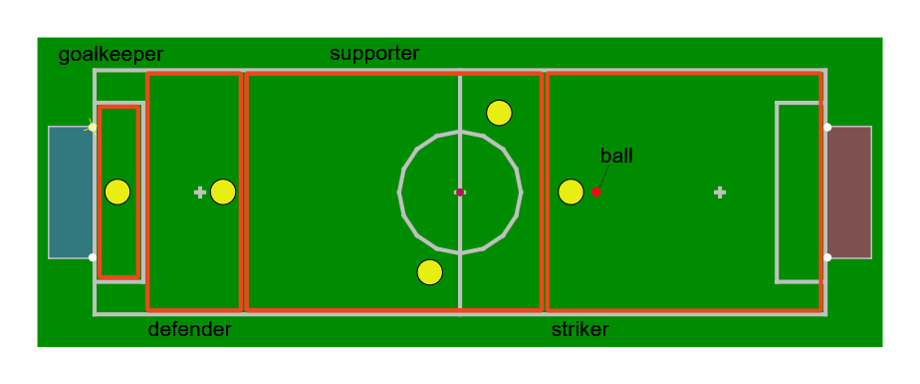
\includegraphics[width=0.9\textwidth]{pics/SPL}
    \centering
    \caption{Roles in SPL}
    \label{fig: SPL}
\end{figure}\\
For the RoboCup at TUM, there are three robots in each team, namely the goal-keeper, defender and striker as shown in \fref{fig: TUM}. The original behavior of these roles are from B-Human CodeRelease in \cite{BHumanCodeRelease2015}.
\begin{figure}[!htb]
    \centering
    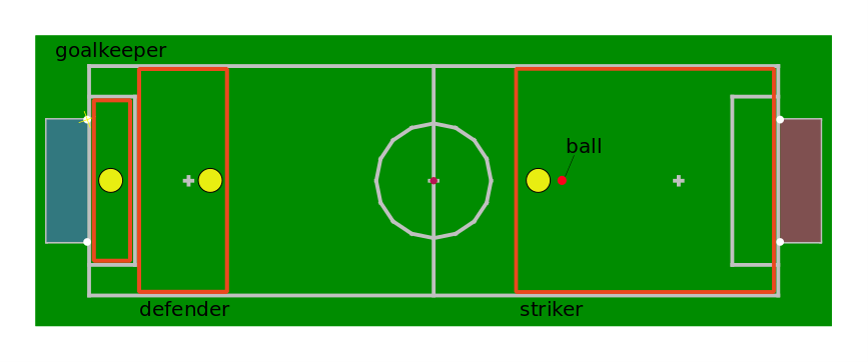
\includegraphics[width=\textwidth]{pics/TUM}
    \caption{Roles at TUM}
    \label{fig: TUM}
\end{figure}

\section{Defender}
\subsection{Defender Behavior}
As shown in the field in \fref{fig: DeFloCha}, defender will always start from one side of the field. Then he will walk to the defense area, face the opponent direction and defend in that area. If the ball is near it in some range, namely smaller than some threshold, he will walk to ball, align to the goal, align behind the ball and kick it out of that region. Then he will go back to the state defend. As a result, the defender will defend in the defense area most of his time as shown in the flow-chart in \fref{fig: DeFloCha}. The original defense area is shown with red rectangle in the left of \fref{fig: DeFloCha}.
\begin{figure}[!htb]
  \centering
  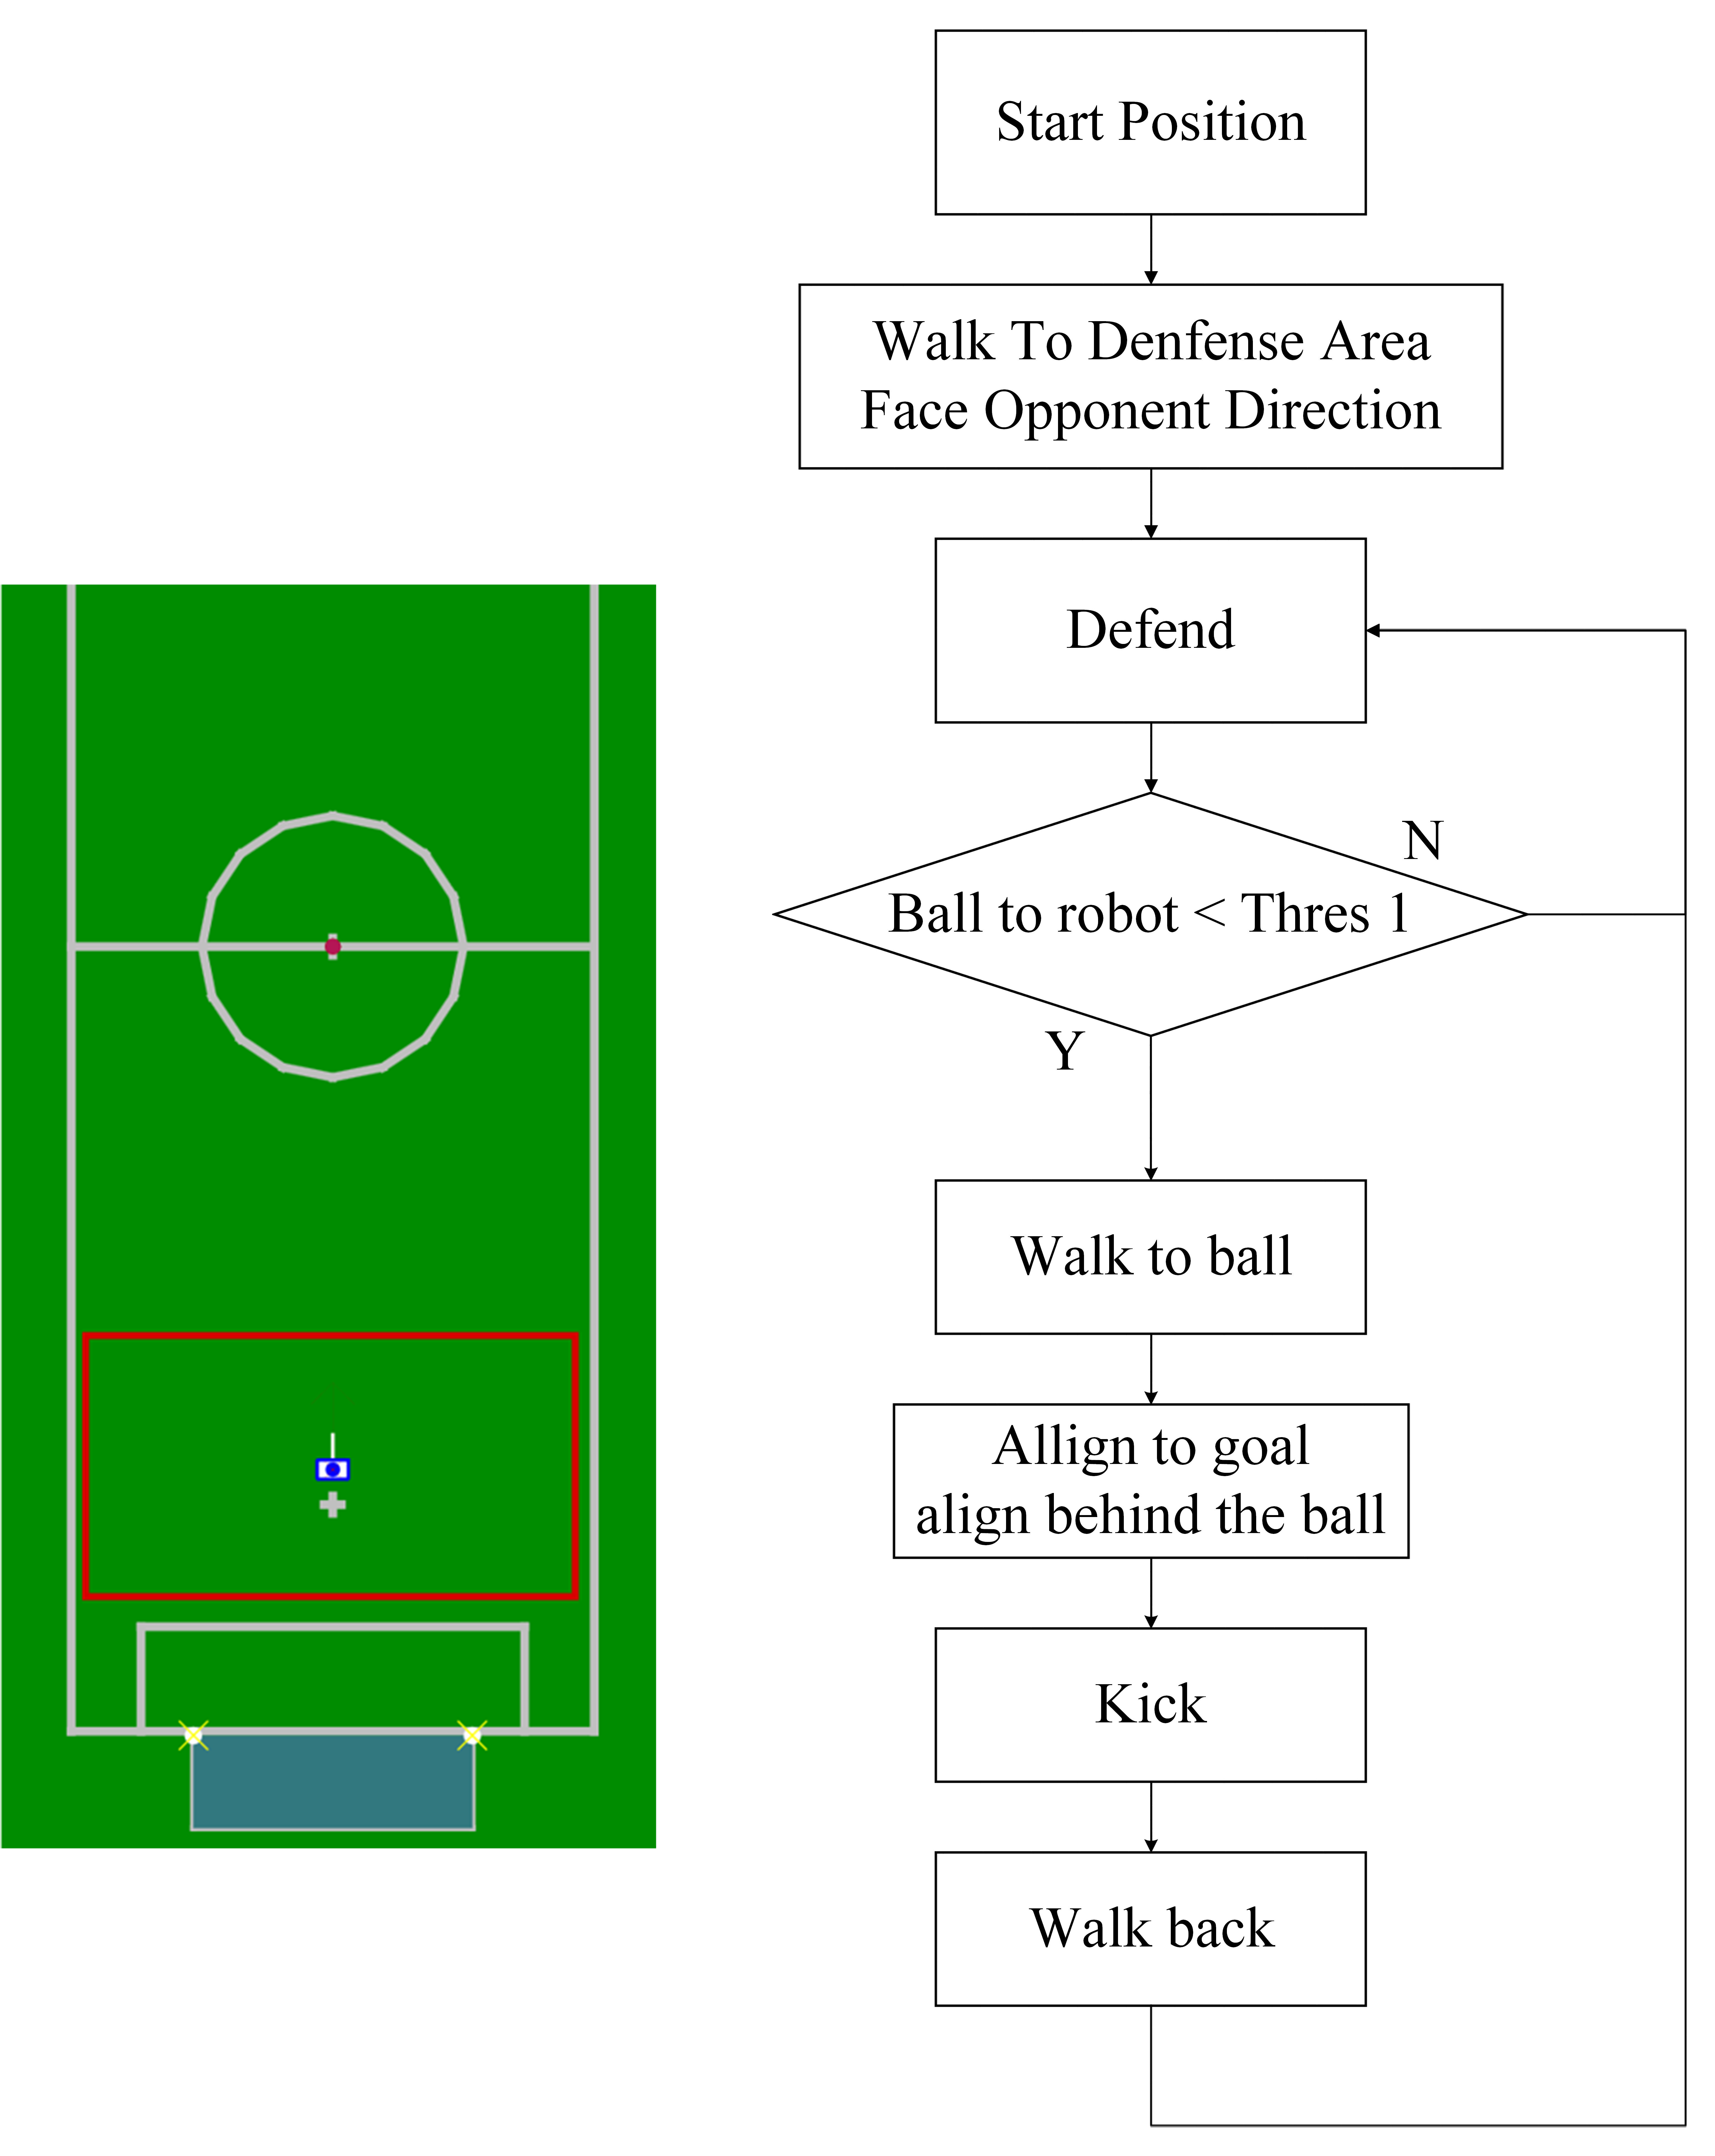
\includegraphics[width=0.8\textwidth]{pics/St_DA}
  \caption{Defender: static defense area and flow chart }
  \label{fig: DeFloCha}
\end{figure}

\subsection{Problems in Defender}
As there are only 3 robots in each team, there is no supporter. The region between the defense area and the center is empty, where is dangerous as no one can stop the opponent striker.

\subsection{Proposed Solution for Defender}
To tactile this problem, a method called ``dynamic defense area'' is proposed as shown in \fref{fig: DefFix}.
\begin{figure}[!htb]
  \centering
  % \includegraphics[scale=0.4]{pics/Dy_DA}
  % \qquad
  % \includegraphics[scale=0.7]{pics/Imp_Def}
  \includegraphics[width=\textwidth]{pics/Dy_DA}
  \caption{Defender: dynamic defense area and flow chart }
  \label{fig: DefFix}
\end{figure}\\
As shown in the flow-chart, the first procedure is the same as before: robots start from one side of the field and go to the defense area to defend there. If ball is near it, it will go and kick it out of that region. What we proposed is another condition, which is highlighted in the flow-chart with red lines: if the ball is far away to the defender, i.e. bigger than some threshold, defender will go to defend in some new region near the center of the field. So the defense area is enlarged until the center of the field. If the ball is suddenly behind the defender, the defender will come back to the original defense area like before. In summary, the defense area is dynamic as it will change according to the distance of the ball and the defender.\\
There are mainly two benefits of the proposed method:
\begin{itemize}
    \item enlarged defense area
    \item compensation for the lack of supporters
\end{itemize}
Even if there are more robots given in the future courses, this behavior can still be kept as the region where the supporters take care is somewhere around the striker, so that they can focusing on supporting on strikers and do not care too much on the field before the center of the field. This can help the team to score more efficiently. The demonstration video for the ``dynamic defense area'' can be found at \url{https://youtu.be/XNjRpqoJ18c}.
\clearpage
\section{Striker}\label{sec:Striker}
\subsection{Striker behavior}
As shown in the flow-chart in \fref{fig: StaStrik}, the striker will always  search for ball, align behind it and kick it in the direction of the center of opponent goal. The direction of the kicking is like the arrow shown in the left part of \fref{fig: StaStrik}.
\begin{figure}[!htb]
  \centering
  % 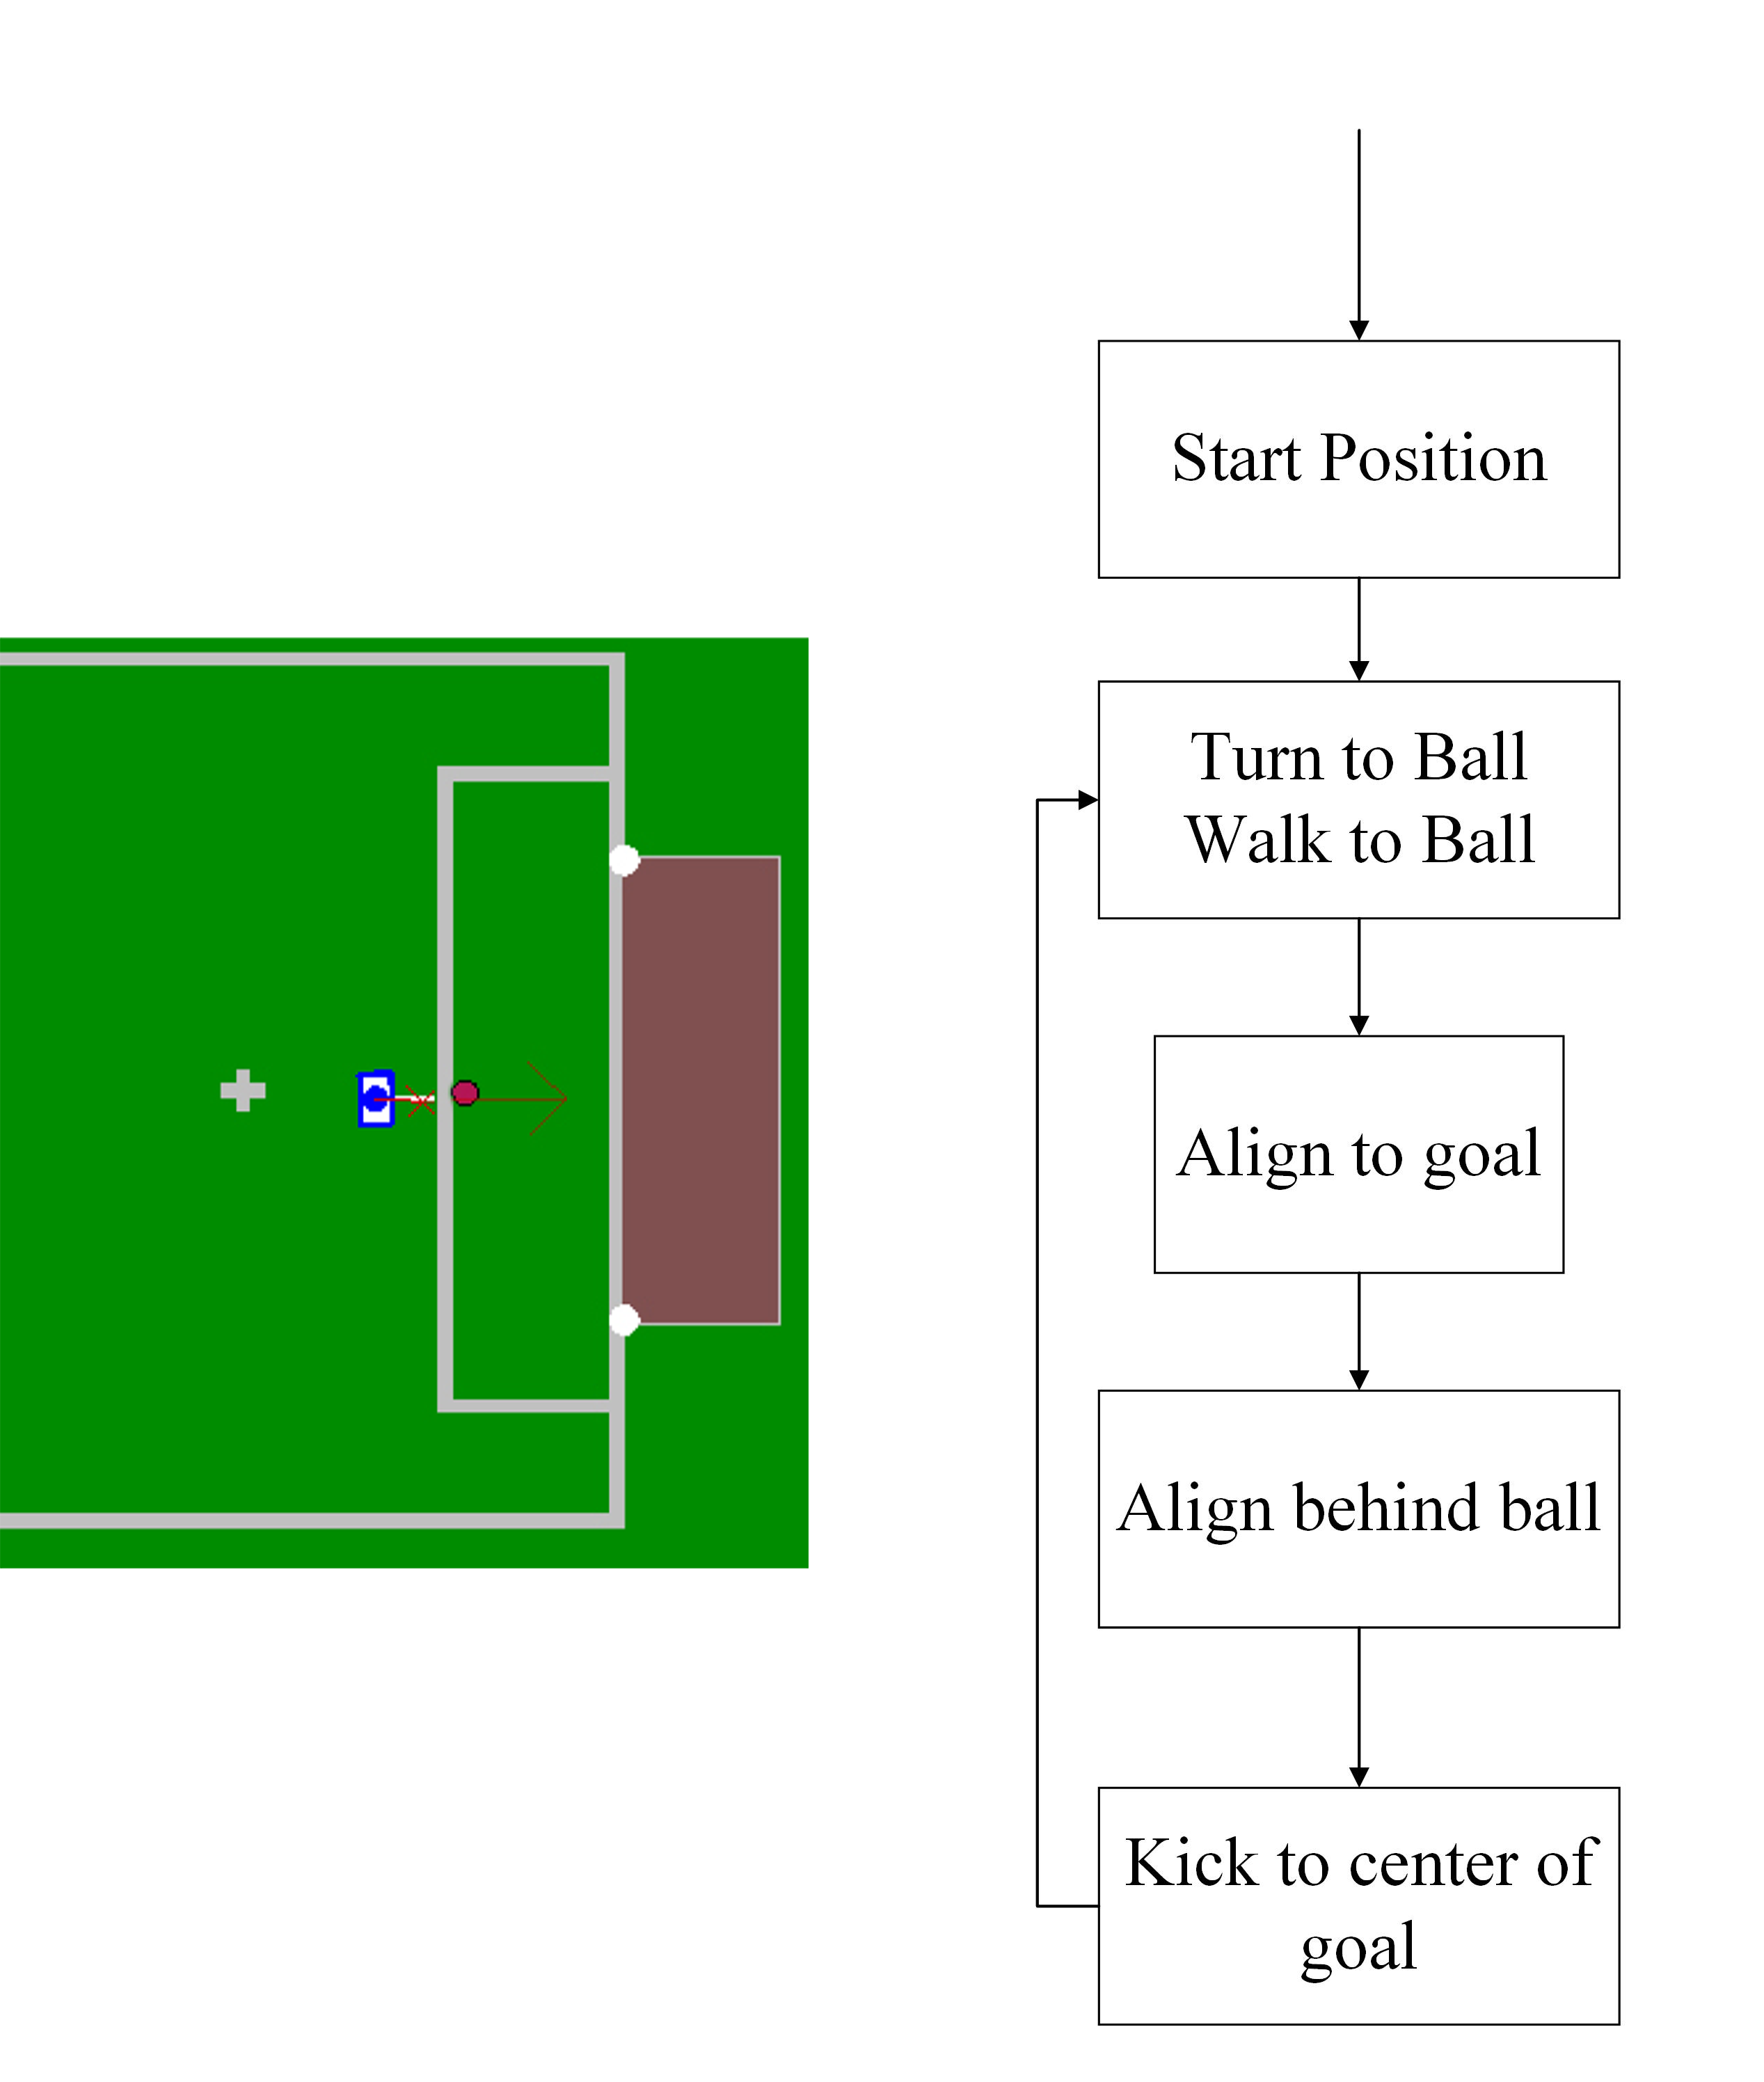
\includegraphics[scale=0.3]{pics/St_Striker}
  % \qquad \qquad \qquad
  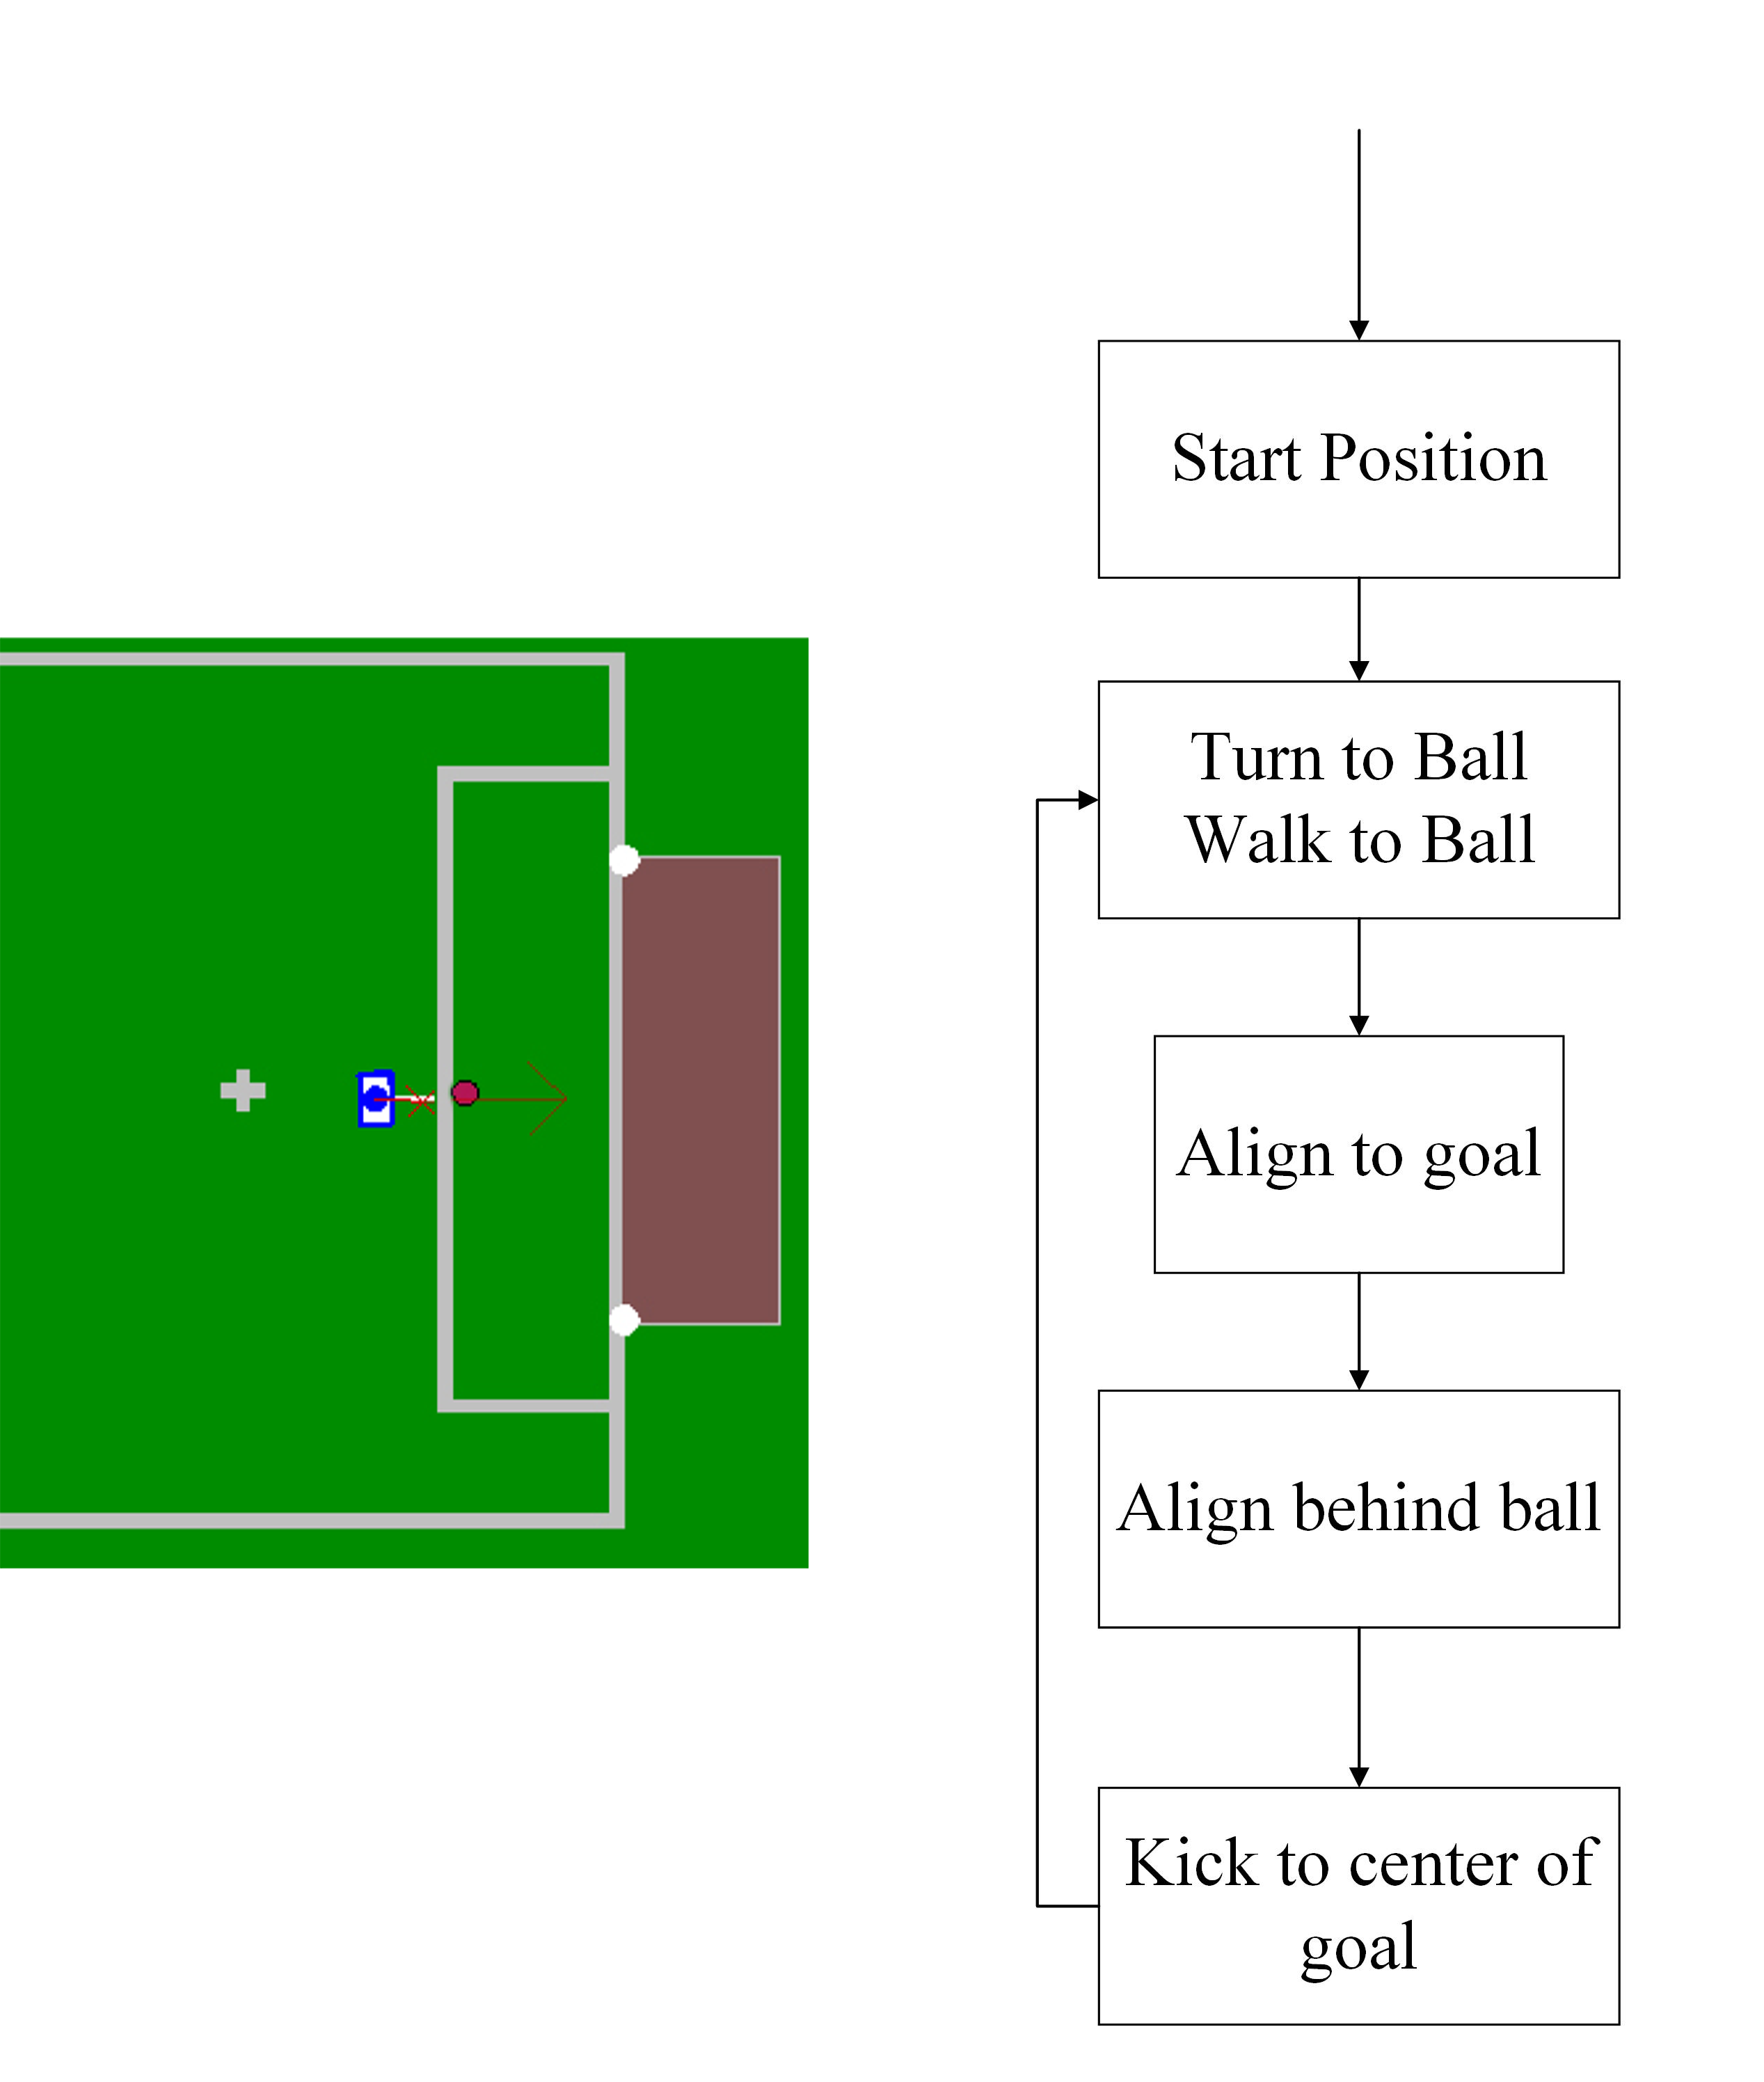
\includegraphics[width=0.7\textwidth]{pics/St_Striker}
  \caption{Striker: static kicking direction and flow chart }
  \label{fig: StaStrik}
\end{figure}

\subsection{Problems in Striker}
The behavior of goal-keeper is to put himself between the ball and the center of the goal. So if the direction of the score kicking is like the arrow shown in \fref{fig: StaStrik}, the ball will stopped by the body of Goalkeeper with high possibility. This is disadvantageous for the team to score the opponent.

\subsection{Proposed Solution for Striker}
To increase the possibility of the scoring kick, a method called ``dynamic kicking direction'' is proposed. The main idea is shown in \fref{fig: DyStrik}.
\begin{figure}[!htb]
  \centering
  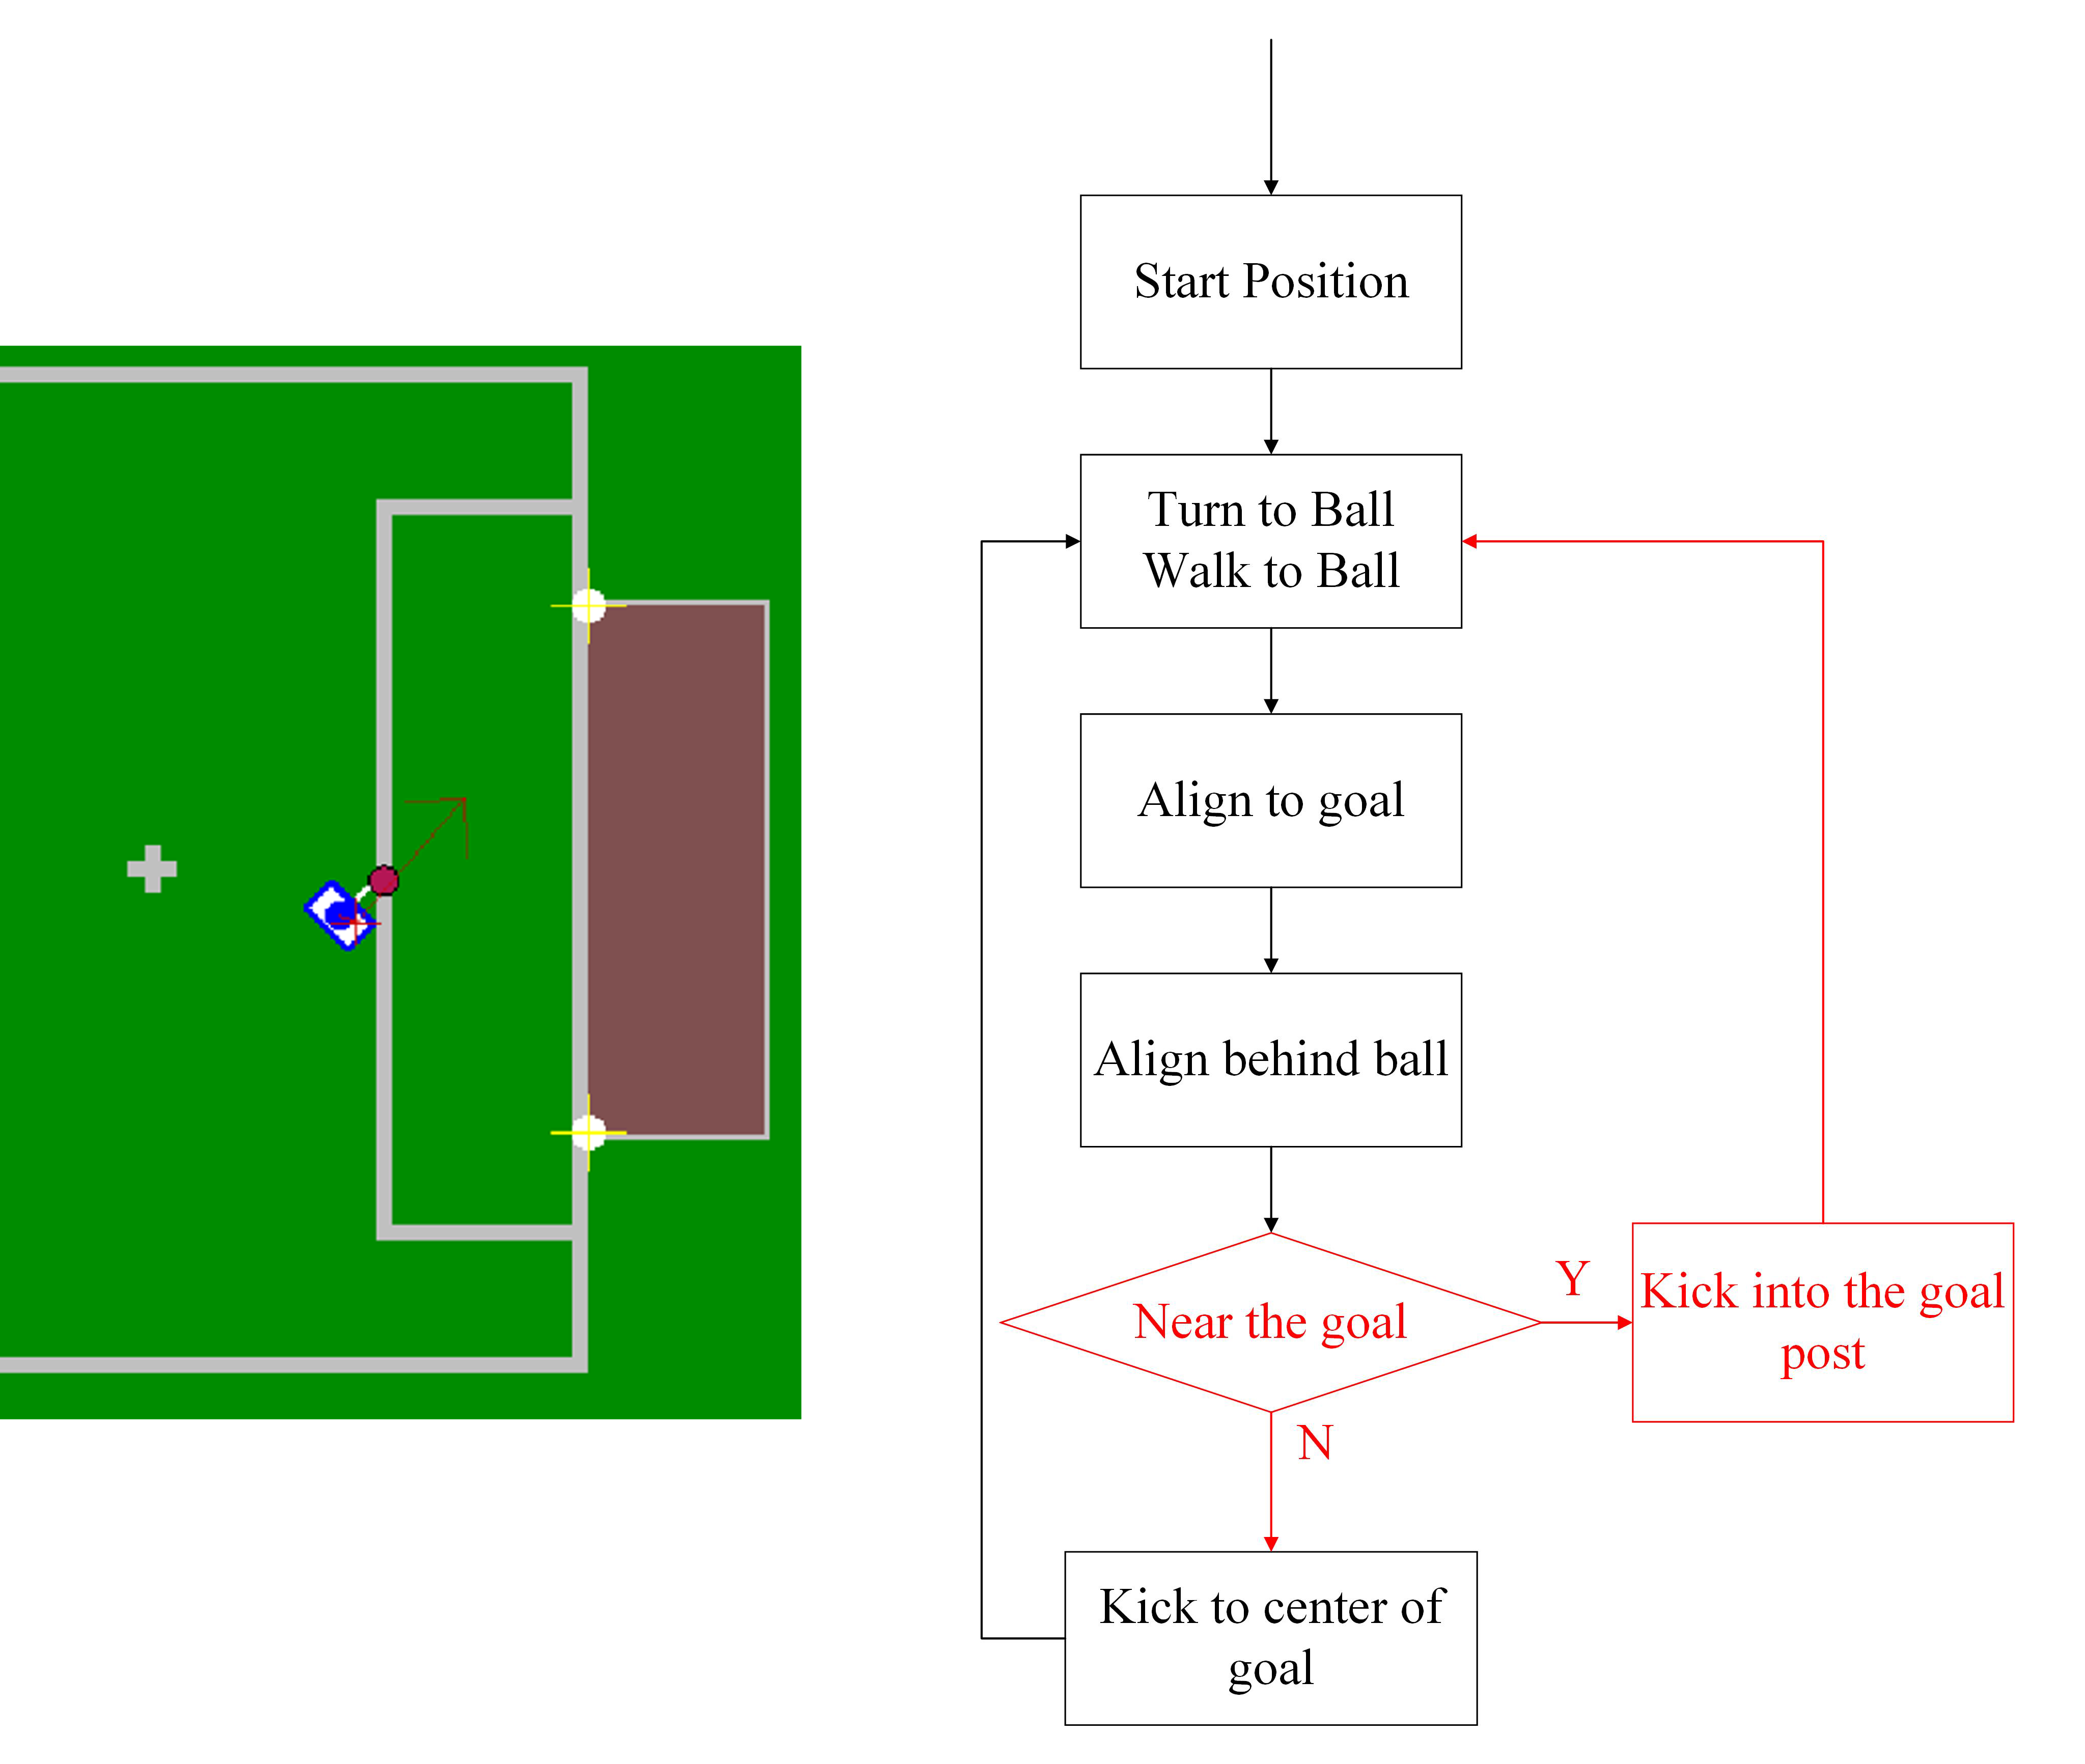
\includegraphics[width=\textwidth]{pics/Dy_Striker}
  % \qquad \qquad
  % \includegraphics[scale=0.7]{pics/Imp_Stri}
  \caption{Striker: dynamic kicking direction and flow chart }
  \label{fig: DyStrik}
\end{figure}\\
The main behavior is identical to the previous. The striker will keep detecting the distance between itself and the center of the opponent goal. If they are near with each other to some threshold, the kicking direction will be changed to the far goal post, rather than the center of the goal, like the arrow direction shown in \fref{fig: DyStrik}.\\
With the proposed method, the striker can score the opponent with higher possibility. The demonstration video for ``dynamic kicking direction'' can be found at \url{https://youtu.be/VrZ4jPr-9Os}.
